\chapter{Desarrollo y Verificación Experimental}\label{sec.ej1:desarrollo}

\section{Arquitectura de la Unidad de Procesamiento Harvard}

La unidad de procesamiento implementada adopta una topología basada en la arquitectura Harvard,
en la cual el bus de datos y el bus de direcciones encuentran físicamente desacoplados. En este esquema,
las consignas de operación llegan a través del bus de control \texttt{regCTRL}, mientras que los
datos externos ingresan por las entradas independientes \texttt{dIN} y \texttt{cIN}. A su
vez, las salidas del circuito proporcionan el dato procesado en \texttt{dOUT}, la dirección correspondiente en
\texttt{aOUT} y el registro de estado o banderas en \texttt{sOUT}.

El diseño fue concebido de manera genérica en SystemVerilog mediante parámetros configurables:
\begin{itemize}
  \item $N$: ancho de palabra del bus de datos (en la presente implementación se fijó en $N = 4$ bits).
  \item $M$: cantidad de bits de direccionamiento del banco de registros (fijado en $M = 2$ bits, lo que permite
        direccionar hasta $2^M = 4$ registros internos, denominados $R_0, R_1, R_2$ y $R_3$).
\end{itemize}

\subsection{Descripción de los bloques constitutivos}

La unidad procesadora se estructura internamente a partir de cuatro componentes principales y tres etapas de
multiplexación:

\begin{enumerate}
  \item Banco de registros (\texttt{ram3port}): constituye la memoria interna del camino de datos. Dispone de dos
        puertos de lectura asíncronos direccionados por las señales \texttt{aAddress} (\texttt{a1}) y \texttt{bAddress}
        (\texttt{a2}), cuyas salidas entregan respectivamente los buses \texttt{aBus} (\texttt{d1}) y \texttt{bBus}
        (\texttt{d2}). La lectura es puramente combinacional. Dispone asimismo de un puerto de escritura direccionado
        por \texttt{dAddress} (\texttt{a3}), el cual captura el valor presente en \texttt{dBus} (\texttt{d3}) durante el
        flanco ascendente de la señal de reloj (\texttt{clk}) únicamente si la señal \texttt{loadEnable} (\texttt{we3})
        se encuentra en nivel alto. \textbf{NOTA:} Se modificó el archivo original provisto por la catedra con el
        objetivo de poder unificar la parametrizacion con los mismos nombres de parametros. Solo se cambió el parametro
        M por el N y viceversa.
  \item Multiplexor de entrada B (\texttt{MUX B}): selecciona la fuente del operando B entre el valor leído del registro
        en \texttt{bBus} y una constante externa provista por \texttt{cIN}. La selección está gobernada por la señal
        \texttt{constInEnable}. La salida de este multiplexor conforma directamente la señal \texttt{dOUT}, que actúa
        como operando para las unidades funcionales.
  \item Unidad aritmético-lógica (\texttt{alu}): procesa los operandos provenientes de \texttt{aOUT} (conectado a
        \texttt{aBus}) y \texttt{dOUT} bajo el control del vector \texttt{aluControl} de 4 bits. Permite ejecutar
        transferencias, incrementos, decrementos, adiciones y sustracciones mediante aritmética en complemento a dos,
        así como funciones lógicas a nivel de bits (AND, OR, XOR y negación). Entrega el resultado de cálculo en
        \texttt{aluOut} y las banderas aritméticas en \texttt{ALUFlags} hacia \texttt{sOUT}, correspondientes a sobreflujo
        ($V$), signo negativo ($N$), cero ($Z$) y acarreo ($C$).
  \item Unidad de corrimiento (\texttt{shifter}): toma como entrada el operando \texttt{dOUT} y aplica operaciones de
        desplazamiento lógico a la izquierda, corrimiento a la derecha con extensión de signo, rotaciones y puesta a cero,
        gobernada por el código \texttt{shifterControl} de 3 bits. Su salida se rotula como \texttt{shifterOut}.
  \item Multiplexor de unidad funcional (\texttt{MUX FU}): arbitra la salida entre la ALU (\texttt{aluOut}) y el
        desplazador (\texttt{shifterOut}) en función del bit de control \texttt{aluEnable}. El dato seleccionado se
        propaga hacia la señal interna \texttt{functionUnitOut}.
  \item Multiplexor de retorno D (\texttt{MUX D}): determina el origen del bus de escritura \texttt{dBus},
        conmutando entre el dato externo entrante por \texttt{dIN} y el resultado producido por la unidad funcional
        en \texttt{functionUnitOut}. Dicha conmutación responde al estado de la señal \texttt{dataInEnable}. El bus
        resultante \texttt{dBus} cierra el lazo de realimentación hacia el puerto de entrada del banco de registros.
\end{enumerate}

\section{Estructura y decodificación de la palabra de control}

La palabra de control \texttt{regCTRL} sintetiza todas las directivas de control del camino de datos en un vector de
$3\times M + 3 + 5 = 14$ bits.

En la figura~\ref{fig.ej1:palabra_control} se ilustra la distribución de los campos dentro de \texttt{regCTRL},
mientras que en la tabla~\ref{tab.ej1:palabra_control} se detalla su asignación a las variables internas del diseño y
sus destinos en el hardware.

\begin{figure}[!ht]
  \centering
  \resizebox{\textwidth}{!}{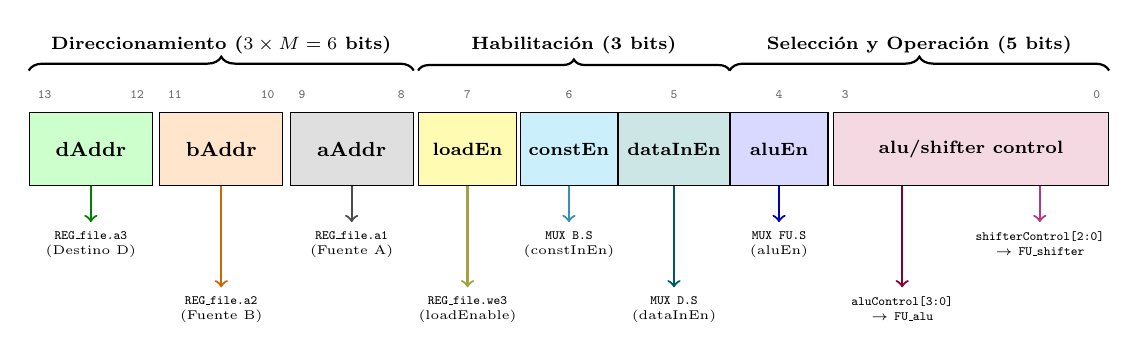
\begin{tikzpicture}[scale=0.92, transform shape,
    box/.style={draw, minimum height=1.0cm, text centered, font=\footnotesize\bfseries},
    bitnum/.style={font=\tiny\ttfamily, text=gray!80!black},
    dest/.style={font=\tiny, align=center, text=black}
  ]

  % Cajas de campos de regCTRL
  \node[box, fill=green!20, minimum width=1.7cm] (daddr) at (0.85, 0) {dAddr};
  \node[box, fill=orange!20, minimum width=1.7cm] (baddr) at (2.65, 0) {bAddr};
  \node[box, fill=gray!25, minimum width=1.7cm] (aaddr) at (4.45, 0) {aAddr};
  \node[box, fill=yellow!30, minimum width=1.35cm] (load) at (6.05, 0) {\scriptsize loadEn};
  \node[box, fill=cyan!20, minimum width=1.35cm] (const) at (7.45, 0) {\scriptsize constEn};
  \node[box, fill=teal!20, minimum width=1.45cm] (din) at (8.90, 0) {\scriptsize dataInEn};
  \node[box, fill=blue!15, minimum width=1.35cm] (aluEn) at (10.35, 0) {\scriptsize aluEn};
  \node[box, fill=purple!15, minimum width=3.8cm] (ctrl) at (13.00, 0) {\scriptsize alu/shifter control};

  % Índices de bits arriba
  \node[bitnum, anchor=south west] at ([yshift=2pt]daddr.north west) {13};
  \node[bitnum, anchor=south east] at ([yshift=2pt]daddr.north east) {12};

  \node[bitnum, anchor=south west] at ([yshift=2pt]baddr.north west) {11};
  \node[bitnum, anchor=south east] at ([yshift=2pt]baddr.north east) {10};

  \node[bitnum, anchor=south west] at ([yshift=2pt]aaddr.north west) {9};
  \node[bitnum, anchor=south east] at ([yshift=2pt]aaddr.north east) {8};

  \node[bitnum, anchor=south] at ([yshift=2pt]load.north) {7};
  \node[bitnum, anchor=south] at ([yshift=2pt]const.north) {6};
  \node[bitnum, anchor=south] at ([yshift=2pt]din.north) {5};
  \node[bitnum, anchor=south] at ([yshift=2pt]aluEn.north) {4};

  \node[bitnum, anchor=south west] at ([yshift=2pt]ctrl.north west) {3};
  \node[bitnum, anchor=south east] at ([yshift=2pt]ctrl.north east) {0};

  % Flechas y destinos abajo - Alternadas limpiamente
  \draw[->, thick, green!50!black] (daddr.south) -- ++(0,-0.5)
    node[below, dest] {\texttt{REG\_file.a3}\\(Destino D)};
  \draw[->, thick, orange!80!black] (baddr.south) -- ++(0,-1.4)
    node[below, dest] {\texttt{REG\_file.a2}\\(Fuente B)};
  \draw[->, thick, black!70] (aaddr.south) -- ++(0,-0.5)
    node[below, dest] {\texttt{REG\_file.a1}\\(Fuente A)};

  \draw[->, thick, yellow!60!black] (load.south) -- ++(0,-1.4)
    node[below, dest] {\texttt{REG\_file.we3}\\(loadEnable)};
  \draw[->, thick, cyan!70!black] (const.south) -- ++(0,-0.5)
    node[below, dest] {\texttt{MUX B.S}\\(constInEn)};
  \draw[->, thick, teal!70!black] (din.south) -- ++(0,-1.4)
    node[below, dest] {\texttt{MUX D.S}\\(dataInEn)};
  \draw[->, thick, blue!70!black] (aluEn.south) -- ++(0,-0.5)
    node[below, dest] {\texttt{MUX FU.S}\\(aluEn)};

  \draw[->, thick, purple!70!black] ([xshift=-0.95cm]ctrl.south) -- ++(0,-1.4)
    node[below, dest] {\texttt{aluControl[3:0]}\\$\rightarrow$ \texttt{FU\_alu}};
  \draw[->, thick, magenta!70!black] ([xshift=0.95cm]ctrl.south) -- ++(0,-0.5)
    node[below, dest] {\texttt{shifterControl[2:0]}\\$\rightarrow$ \texttt{FU\_shifter}};

  % Llaves superiores agrupadoras
  \draw[decorate, decoration={brace, amplitude=5pt, raise=14pt}, thick]
    (daddr.west |- 0,0.55) -- (aaddr.east |- 0,0.55)
    node[midway, above=18pt, font=\scriptsize\bfseries] {Direccionamiento ($3\times M = 6$ bits)};

  \draw[decorate, decoration={brace, amplitude=4pt, raise=14pt}, thick]
    (load.west |- 0,0.55) -- (din.east |- 0,0.55)
    node[midway, above=18pt, font=\scriptsize\bfseries] {Habilitación (3 bits)};

  \draw[decorate, decoration={brace, amplitude=5pt, raise=14pt}, thick]
    (aluEn.west |- 0,0.55) -- (ctrl.east |- 0,0.55)
    node[midway, above=18pt, font=\scriptsize\bfseries] {Selección y Operación (5 bits)};

\end{tikzpicture}
}
  \caption{Estructura de partición de la palabra de control \texttt{regCTRL[13:0]}.}
  \label{fig.ej1:palabra_control}
\end{figure}

\begin{table}[!ht]
  \centering
  \small
  \caption{Mapeo de la palabra de control en las variables internas de la unidad.}
  \label{tab.ej1:palabra_control}
  \resizebox{\textwidth}{!}{%
  \begin{tabular}{cccll}
    \toprule
    Rango de bits & Variable interna & Ancho & Función principal & Módulo de destino \\
    \midrule
    \texttt{[13:12]} & \texttt{dAddress}       & 2 bits & Dirección de registro destino       & \texttt{REG\_file.a3} \\
    \texttt{[11:10]} & \texttt{bAddress}       & 2 bits & Dirección de registro fuente B      & \texttt{REG\_file.a2} \\
    \texttt{[9:8]}   & \texttt{aAddress}       & 2 bits & Dirección de registro fuente A      & \texttt{REG\_file.a1} \\
    \texttt{[7]}     & \texttt{loadEnable}     & 1 bit  & Habilitación de escritura           & \texttt{REG\_file.we3} \\
    \texttt{[6]}     & \texttt{constInEnable}  & 1 bit  & Selección de constante vs registro  & \texttt{MUX B.S} \\
    \texttt{[5]}     & \texttt{dataInEnable}   & 1 bit  & Selección de dato externo vs cálculo& \texttt{MUX D.S} \\
    \texttt{[4]}     & \texttt{aluEnable}      & 1 bit  & Selección ALU vs Desplazador        & \texttt{MUX FU.S} \\
    \texttt{[3:0]}   & \texttt{aluControl}     & 4 bits & Operación de la ALU                 & \texttt{FU\_alu.ALUControl} \\
    \texttt{[2:0]}   & \texttt{shifterControl} & 3 bits & Operación del desplazador           & \texttt{FU\_shifter.S} \\
    \bottomrule
  \end{tabular}%
  }
\end{table}

\section{Síntesis lógica y esquemático RTL}

Para corroborar la topología del circuito y examinar la distribución efectiva de las señales de control hacia cada
instancia y multiplexor, se llevó a cabo la síntesis lógica.

En la figura~\ref{fig.ej1:rtl_schematic} se expone el diagrama RTL generado. En él se aprecia de manera
directa cómo la palabra de control \texttt{regCTRL} se descompone en sus respectivos rebanados de bits.
Desde dichos nodos, las líneas de control se propagan de forma unívoca:
\begin{itemize}
  \item Las variables de direccionamiento \texttt{aAddress}, \texttt{bAddress} y \texttt{dAddress}, junto con la señal
        de habilitación de escritura \texttt{loadEnable}, ingresan al banco de registros \texttt{REG\_file}.
  \item La variable \texttt{aluControl} se conecta directamente a la entrada \texttt{ALUControl} de la instancia
        \texttt{FU\_alu}.
  \item La variable \texttt{shifterControl} ingresa a la entrada de selección \texttt{S} de la unidad
        \texttt{FU\_shifter}.
  \item Las variables \texttt{constInEnable}, \texttt{aluEnable} y \texttt{dataInEnable} conmutan las entradas de
        control \texttt{S} de los multiplexores \texttt{MUX B}, \texttt{MUX FU} y \texttt{MUX D}, respectivamente.
  \item Se visualiza con total claridad el lazo cerrado de realimentación: el bus \texttt{dBus}, generado por la salida
        del multiplexor \texttt{MUX D}, regresa hacia la entrada de datos de escritura \texttt{d3} del banco de
        registros.
\end{itemize}

\begin{figure}[!ht]
  \centering
  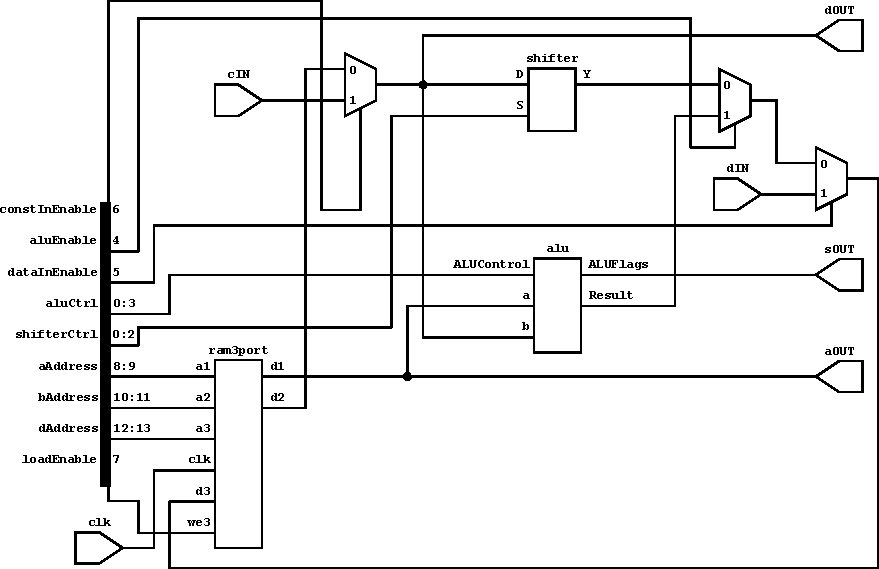
\includegraphics[width=\textwidth]{sources/up_harvard.pdf}
  \caption{Esquemático RTL del módulo \texttt{up\_harvard} sintetizado con Yosys.}
  \label{fig.ej1:rtl_schematic}
\end{figure}

\section{Verificación mediante simulación}

La verificación del camino de datos se efectuó a través del banco de pruebas. Cada vector del banco de prueba posee una
longitud de 22 bits, estructurado como la concatenación \texttt{\{regCTRL, cIN, dIN\}}. El período del reloj de prueba
se fijó en $\qty{20}{\nano\second}$.

El plan de prueba abarca una secuencia de 8 ciclos de reloj ($T_0$ a $T_7$) orientados a validar la carga inicial,
dos operaciones aritméticas fundamentales, una operación de corrimiento y las lecturas de verificación correspondientes:

\begin{enumerate}
  \item Ciclo $T_0$: Carga inicial en el registro $R_0$.  Se aplica \texttt{dIN = 5}, con \texttt{dAddress = 0},
    \texttt{loadEnable = 1} y \texttt{dataInEnable = 1}. En el flanco ascendente de reloj, el valor 5 queda almacenado
    en $R_0$.
  \item Ciclo $T_1$: Carga inicial en el registro $R_1$.  Se aplica \texttt{dIN = 3}, con \texttt{dAddress = 1},
    \texttt{loadEnable = 1} y \texttt{dataInEnable = 1}. En el flanco ascendente de reloj, el valor 3 queda almacenado
    en $R_1$.
  \item Ciclo $T_2$: \textbf{Primera operación aritmética (Suma)}.  Se ejecuta la adición $R_2 \leftarrow R_0 + R_1$.
    Los puertos de lectura seleccionan $R_0$ (\texttt{aAddress = 0}) y $R_1$ (\texttt{bAddress = 1}), entregando
    $\texttt{aBus} = 5$ y $\texttt{bBus} = 3$. Con \texttt{constInEnable = 0}, la entrada B de la ALU recibe
    $\texttt{dOUT} = 3$. Se configura \texttt{aluEnable = 1} y \texttt{aluControl = 0010b} (operación $A + B$). La ALU
    genera $\texttt{aluOut} = 5 + 3 = 8$. Con \texttt{dataInEnable = 0}, este resultado se transfiere a $\texttt{dBus} =
    8$ y se escribe en $R_2$ (\texttt{dAddress = 2}, \texttt{loadEnable = 1}) en el flanco de subida siguiente. Las
    banderas generadas en \texttt{sOUT} son \texttt{0100b}, indicando la activación de la bandera de signo negativo ($N
    = 1$), debido a que en representación con signo de 4 bits el patrón \texttt{1000b} posee su bit más significativo en
    1.
  \item Ciclo $T_3$: Verificación de lectura de la suma.  Se configura \texttt{bAddress = 2} con \texttt{constInEnable =
    0} y \texttt{loadEnable = 0}. La salida \texttt{dOUT} refleja de inmediato el contenido de $R_2$ ($8$), confirmando
    que el valor fue almacenado correctamente.
  \item Ciclo $T_4$: \textbf{Segunda operación aritmética (Resta)}.  Se ejecuta la sustracción con operando constante
    $R_2 \leftarrow R_2 - cIN$, empleando $cIN = 2$ (\texttt{0010b}).  Se direcciona \texttt{aAddress = 2} ($R_2 = 8$) y
    se activa \texttt{constInEnable = 1}, de modo que $\texttt{dOUT} = 2$.  El control de la ALU se establece en
    \texttt{aluControl = 0101b}, correspondiente a la operación aritmética de sustracción $A + \sim B + 1$. El resultado
    producido es $\texttt{aluOut} = 8 - 2 = 6$ (\texttt{0110b}). Al estar habilitada la escritura sobre $R_2$
    (\texttt{dAddress = 2}, \texttt{loadEnable = 1}), el nuevo valor 6 se registra en el flanco de subida. Las banderas
    resultantes son \texttt{0001b}, encendiendo la bandera de acarreo ($C = 1$), lo cual certifica que no existió
    condición de préstamo negativo en la resta.
  \item Ciclo $T_5$: Verificación de lectura de la resta.  Se direcciona nuevamente $R_2$ hacia el bus B
    (\texttt{bAddress = 2}) con \texttt{constInEnable = 0}. La salida \texttt{dOUT} muestra el valor 6.
  \item Ciclo $T_6$: Operación de corrimiento a la izquierda.  Se aplica un desplazamiento lógico sobre $R_2$: $R_2
    \leftarrow R_2 \ll 1$. Con \texttt{bAddress = 2} y \texttt{constInEnable = 0}, la unidad de corrimiento recibe el
    valor 6 por \texttt{dOUT}. Se configura \texttt{shifterControl = 001b} (SHL) y se desactiva la ALU
    (\texttt{aluEnable = 0}), permitiendo el paso de \texttt{shifterOut} a través de \texttt{MUX FU}. El valor
    resultante es $\texttt{fuOut} = 6 \ll 1 = 12$ (\texttt{1100b}), el cual se escribe en $R_2$ al flanco de subida.
  \item Ciclo $T_7$: Verificación final de corrimiento.  Se lee el registro $R_2$ en la salida \texttt{dOUT},
    comprobando el valor final 12 (\texttt{1100b}).
\end{enumerate}

\begin{figure}[!ht]
  \centering
  \resizebox{\textwidth}{!}{\begin{tikztimingtable}[
    timing/slope=0.05,
    timing/coldist=4pt,
    xscale=2.2,
    yscale=1.1,
    timing/dslope=0.1
]
  \texttt{clk}            & 16{C} \\
  \texttt{datain[3:0]}    & 2D{5} 2D{3} 12D{0} \\
  \texttt{constin[3:0]}   & 8D{0} 2D{2} 6D{0} \\
  \texttt{control[13:0]}  & 2D{00A0} 2D{10A0} 2D{2492} 2D{3B00} 2D{2ED5} 2D{3B00} 2D{2A81} 2D{3B00} \\
  \texttt{dataout[3:0]}   & 1X 3D{5} 2D{3} 2D{8} 2D{2} 3D{6} 3D{12} \\
  \texttt{addressout[3:0]}& 1X 5D{5} 2X 1D{8} 1D{6} 2X 1D{6} 1D{12} 2X \\
  \texttt{flags[3:0]}     & 1X 3D{0000} 2D{0100} 2X 2D{0001} 2X 1D{0000} 1D{0100} 2X \\
\extracode
  % Fondo sombreado alternado para distinguir cada ciclo de reloj
  \begin{pgfonlayer}{background}
    \foreach \t in {0, 4, 8, 12} {
      \pgfmathsetmacro{\tend}{\t+2}
      \fill[blue!4] (\t, 2.2) rectangle (\tend, -14.5);
    }
    \vertlines[gray!40, dashed, line width=0.5pt]{0, 2, ..., 16}
  \end{pgfonlayer}

  % Tiempos numéricos (eje temporal superior, cada 20 ns)
  \foreach \i in {0, ..., 8} {
    \pgfmathsetmacro{\x}{\i * 2}
    \pgfmathsetmacro{\tval}{\i * 20}
    \node[font=\sffamily\tiny, text=gray!80!black, anchor=south] at (\x, 4.4) {$\pgfmathprintnumber{\tval}$\,ns};
  }

  % Ciclos T0 a T7 y descripción de operaciones
  \foreach \i/\desc in {
    0/{Carga $R_0$},
    1/{Carga $R_1$},
    2/{Suma},
    3/{Lectura},
    4/{Resta},
    5/{Lectura},
    6/{SHL},
    7/{Lectura}
  } {
    \pgfmathsetmacro{\xc}{\i * 2 + 1}
    \node[font=\sffamily\scriptsize\bfseries, blue!80!black, anchor=south] at (\xc, 3.4) {$T_\i$};
    \node[font=\sffamily\tiny, text=darkgray, anchor=south] at (\xc, 2.4) {\desc};
  }
\end{tikztimingtable}
}
  \caption{Cronograma de señales de la simulación temporal en el banco de pruebas.}
  \label{fig.ej1:simulacion}
\end{figure}

En la tabla~\ref{tab.ej1:resumen_test} se resume la correlación entre las palabras de control aplicadas, las señales
internas y los resultados verificados en el camino de datos durante cada ciclo de prueba.

\begin{table}[!ht]
  \centering
  \small
  \caption{Resumen de la secuencia de prueba y resultados de simulación.}
  \label{tab.ej1:resumen_test}
  \resizebox{\textwidth}{!}{%
  \begin{tabular}{cclcccccc}
    \toprule
    Ciclo & Tiempo [\unit{\nano\second}] & Operación ejecutada & \texttt{regCTRL} & \texttt{dIN} & \texttt{cIN} & \texttt{dOUT} & \texttt{dBus} & Banderas \\
    \midrule
    $T_0$ & $0 - 20$   & Carga $R_0 \leftarrow 5$          & \texttt{00A0h} & 5 & 0 & -- & 5  & -- \\
    $T_1$ & $20 - 40$  & Carga $R_1 \leftarrow 3$          & \texttt{04A0h} & 3 & 0 & -- & 3  & -- \\
    $T_2$ & $40 - 60$  & Suma: $R_2 \leftarrow R_0 + R_1$   & \texttt{2492h} & 0 & 0 & 3  & 8  & \texttt{0100b} ($N=1$) \\
    $T_3$ & $60 - 80$  & Lectura $R_2$                     & \texttt{3B00h} & 0 & 0 & 8  & -- & -- \\
    $T_4$ & $80 - 100$ & Resta: $R_2 \leftarrow R_2 - cIN$  & \texttt{2ED5h} & 0 & 2 & 2  & 6  & \texttt{0001b} ($C=1$) \\
    $T_5$ & $100 - 120$& Lectura $R_2$                     & \texttt{3B00h} & 0 & 0 & 6  & -- & -- \\
    $T_6$ & $120 - 140$& Corrimiento: $R_2 \leftarrow R_2 \ll 1$ & \texttt{2AA1h} & 0 & 0 & 6  & 12 & \texttt{0100b} ($N=1$) \\
    $T_7$ & $140 - 160$& Lectura $R_2$                     & \texttt{3B00h} & 0 & 0 & 12 & -- & -- \\
    \bottomrule
  \end{tabular}%
  }
\end{table}
